% ICML 2025 Paper Template for Overleaf
% Auto-generated by Anonymous Research Pipeline
%
% Instructions:
% 1. Upload this folder to Overleaf
% 2. Ensure icml2025.sty is in the same directory
% 3. Compile with pdfLaTeX
%
\documentclass{article}

% ICML 2025 style - download from https://icml.cc/Conferences/2025/StyleAuthorInstructions
% Comment out the next line if icml2025.sty is not available
\IfFileExists{icml2025.sty}{\usepackage{icml2025}}{}

% Standard packages
\usepackage{microtype}
\usepackage{graphicx}
\usepackage{subfigure}
\usepackage{booktabs}
\usepackage{hyperref}
\usepackage{amsmath}
\usepackage{amssymb}
\usepackage{algorithm}
\usepackage{algorithmic}

% For better table formatting
\usepackage{multirow}
\usepackage{makecell}

% Bibliography
\usepackage{natbib}

% Fallback if ICML style not present
\makeatletter
\@ifundefined{icmltitle}{%
  \newcommand{\icmltitle}[1]{\title{#1}}
  \newcommand{\icmltitlerunning}[1]{}
  \newenvironment{icmlauthorlist}{}{}
  \newcommand{\icmlauthor}[2]{}
  \newcommand{\icmlaffiliation}[2]{}
  \newcommand{\icmlcorrespondingauthor}[2]{}
  \newcommand{\icmlkeywords}[1]{}
  \newcommand{\printAffiliationsAndNotice}[1]{}
}{}
\makeatother

% ============================================================================
% DOCUMENT METADATA
% ============================================================================

\icmltitlerunning{Gradient Subspace Analysis Requirements}

\begin{document}

\twocolumn[
\icmltitle{Measurement Requirements for Gradient Subspace Analysis in Spurious Correlation Robustification}

% Author information - fill before submission
\begin{icmlauthorlist}
\icmlauthor{Anonymous Author}{}
\end{icmlauthorlist}

\icmlaffiliation{}{Anonymous Institution}

\icmlcorrespondingauthor{Anonymous Author}{anonymous@anonymous.org}

\icmlkeywords{Machine Learning, Spurious Correlations, Gradient Analysis, ICML}

\vskip 0.3in
]

% Print title but hide author info for review
\printAffiliationsAndNotice{}

% ============================================================================
% ABSTRACT
% ============================================================================

\begin{abstract}
Neural networks exploit spurious correlations in training data, and gradient-based interventions promise single-run robustification without group labels. We test the foundational assumption underlying Progressive Gradient Orthogonalization: that early training gradients capture spurious feature directions. Our experiments on Waterbirds reveal a critical measurement challenge---naive gradient subspace accumulation produces representations too low-rank to distinguish spurious from core directions. With one gradient per epoch, we observe both alignments at approximately 0.05, indistinguishable from random projection in a 25-million-parameter space. This null result stems from insufficient accumulation density rather than absence of the hypothesized effect. We establish minimum requirements for valid gradient subspace analysis: multi-batch accumulation is necessary to achieve sufficient rank for meaningful directional measurement. Our findings provide methodological guidance for gradient-based robustification research: validate measurement apparatus before testing intervention hypotheses.

\end{abstract}

% ============================================================================
% MAIN CONTENT
% ============================================================================

\section{Introduction}

Gradient-based interventions for spurious correlation robustness promise single-run training without group labels---but our experiments reveal a critical measurement challenge: naive gradient subspace accumulation produces representations too low-rank to distinguish spurious from core feature directions. When we expected clear separation ($>$70\% spurious alignment vs $<$30\% core alignment based on simplicity bias theory), we observed both at approximately 5\%---essentially indistinguishable from random projection.

This finding matters because methods claiming to exploit training dynamics for robustness may be measuring noise rather than meaningful signal. Without understanding minimum requirements for gradient subspace analysis, researchers risk investing effort in fundamentally flawed approaches that cannot be validated.

\subsection{The Problem}

Deep neural networks trained with empirical risk minimization (ERM) reliably learn spurious correlations---shortcuts that achieve low training loss but fail on minority groups. On the Waterbirds benchmark, ERM models learn to associate waterbirds with water backgrounds (95\% correlation in training data), achieving only 60\% worst-group accuracy when waterbirds appear on land backgrounds.

Existing solutions require resources unavailable in many practical settings. Group DRO needs group annotations during training. Just Train Twice (JTT) requires two complete training runs. Deep Feature Reweighting (DFR) needs held-out data with group labels for last-layer retraining. The promise of training dynamics exploitation---intervening on gradients during a single training run without any labels---remains unrealized.

The deeper problem is that we do not know whether gradient subspace methods can even distinguish spurious from core feature directions. Simplicity bias theory predicts that early training gradients should point toward spurious (simpler) features, but this has been assumed rather than measured. Before designing gradient orthogonalization methods, we need validated measurement apparatus.

\subsection{Our Investigation}

We tested the foundational assumption underlying Progressive Gradient Orthogonalization (PGO): that early gradient subspaces primarily capture spurious feature directions. We trained ResNet-50 on Waterbirds, accumulated gradients during epochs 1-10, computed a top-50 SVD subspace, and measured alignment with spurious (background-varying) and core (bird-type-varying) gradient directions.

The result was unexpected. Both alignments registered at approximately 0.05---far below the 0.70 and 0.30 thresholds predicted by simplicity bias theory, and statistically indistinguishable from each other. Investigation revealed the cause: accumulating only one gradient per epoch produced a 10-dimensional subspace in a 25-million-parameter space. This is insufficient to capture meaningful variance in any direction. The measurement apparatus failed before the hypothesis could be tested.

\subsection{Contributions}

This investigation yields a methodological constraint rather than a positive result:

\begin{enumerate}
    \item We demonstrate that gradient subspace analysis in high-dimensional parameter spaces requires sufficient sample density---single gradients per epoch produce subspaces too low-rank for meaningful directional analysis.
    \item We document the minimum requirements for valid gradient subspace measurement: multi-batch accumulation within early epochs, not single-batch per epoch sampling.
    \item We provide a template for future gradient-based robustification work to validate measurement apparatus before testing hypotheses.
\end{enumerate}

The Progressive Gradient Orthogonalization hypothesis remains unverified. What we establish is what valid testing requires. Future work should accumulate gradients across all batches during early epochs using streaming SVD before attempting to measure spurious-core separation.

\section{Related Work}

We position our investigation at the intersection of spurious correlation robustification and training dynamics analysis. Prior work establishes the phenomenon and develops mitigation strategies; we test whether gradient-based intervention is even measurable.

\subsection{Spurious Correlation and Shortcut Learning}

\citet{geirhos2020shortcut} formalized the taxonomy of shortcut learning in deep neural networks, documenting how models exploit dataset biases rather than learning intended features. Their survey established the scope of the problem but focused on detection rather than intervention.

\citet{sagawa2020distributionally} introduced Group DRO and the Waterbirds/CelebA benchmarks, enabling standardized evaluation of worst-group accuracy. Group DRO requires group annotations during training---a resource often unavailable in practice. This limitation motivates annotation-free approaches.

\textbf{Our complement:} These works establish the phenomenon exists. We test whether gradient subspace methods can measure it during training.

\subsection{Annotation-Free Robustification}

\citet{liu2021just} developed Just Train Twice (JTT), a two-stage approach that identifies spurious-reliant samples via training dynamics, then upweights them. JTT removes the need for group labels but requires two complete training runs.

\citet{kirichenko2023last} showed that last-layer retraining (Deep Feature Reweighting, DFR) suffices for robustification, suggesting pretrained representations already contain core features. DFR requires held-out data with group labels for reweighting.

\citet{creager2021environment} introduced EIIL, inferring pseudo-environments from training dynamics without explicit group annotations. Like JTT, this operates at the sample level rather than gradient level.

\textbf{The gap we address:} All these methods operate on samples or final representations. None validates whether gradient directions themselves can distinguish spurious from core features---the assumption underlying gradient-based intervention.

\subsection{Simplicity Bias and Training Dynamics}

\citet{shah2020pitfalls} documented simplicity bias: neural networks trained with SGD preferentially learn simpler features first. Since spurious correlations often involve simpler patterns (background texture vs.\ object shape), this explains early spurious feature acquisition.

\citet{nagarajan2021understanding} analyzed failure modes of out-of-distribution generalization, connecting training dynamics to generalization failure. Their theoretical analysis suggests early gradients favor low-complexity solutions.

\textbf{The assumption we test:} These works predict that early gradient subspaces should predominantly capture spurious directions. We attempt to measure this directly and find the measurement apparatus itself requires validation.

\subsection{Gradient-Based Representation Analysis}

Gradient analysis methods have been applied to interpretability \citep{simonyan2014deep, sundararajan2017axiomatic} and adversarial robustness \citep{madry2018towards}. These works analyze gradients with respect to inputs, not parameter-space subspaces.

Parameter-space gradient subspace analysis appears primarily in optimization literature (incremental PCA, streaming SVD) rather than robustification. We bridge this gap by applying subspace methods to spurious correlation measurement.

\textbf{Our contribution:} We identify minimum requirements for gradient subspace methods: sufficient accumulation density relative to parameter dimensionality. Single gradients per epoch produce subspaces too low-rank to measure anything meaningful in 25M-parameter models.

\subsection{Position Summary}

Our work complements rather than supersedes existing approaches. We do not claim gradient-based robustification is impossible---we identify what valid measurement requires. Future gradient orthogonalization methods should validate their measurement apparatus using the requirements we establish before testing intervention hypotheses.

\section{Methodology}

Our methodology tests whether gradient subspace accumulation can distinguish spurious from core feature directions. We design a measurement apparatus and document its requirements for valid operation.

\subsection{Problem Formulation}

Let $f_\theta: \mathcal{X} \to \mathcal{Y}$ be a neural network with parameters $\theta \in \mathbb{R}^d$. During training, the gradient $\nabla_\theta \mathcal{L}$ provides a $d$-dimensional direction of parameter change.

\textbf{Hypothesis:} Under simplicity bias, early training gradients point predominantly toward spurious feature directions. Accumulating these gradients into a subspace $S$ via SVD should yield high alignment with spurious directions and low alignment with core directions.

\textbf{Measurement goal:} Quantify alignment between gradient subspace $S$ and spurious/core feature directions.

\subsection{Gradient Subspace Accumulation}

We accumulate gradients during early training epochs and compute a principal subspace via SVD.

\begin{algorithm}[h]
\caption{Gradient Subspace Computation}
\begin{algorithmic}[1]
\REQUIRE Model $\theta$, epochs $T_{\text{acc}}$, rank $k$
\ENSURE Subspace $S \in \mathbb{R}^{d \times k}$
\STATE $G \leftarrow$ empty matrix
\FOR{epoch $t = 1$ to $T_{\text{acc}}$}
    \FOR{batch in dataloader}
        \STATE compute loss $\mathcal{L}(\theta)$
        \STATE $g_t \leftarrow \text{flatten}(\nabla_\theta \mathcal{L})$
        \STATE append $g_t$ to $G$
    \ENDFOR
\ENDFOR
\STATE $U, \Sigma, V^T \leftarrow \text{SVD}(G)$
\STATE $S \leftarrow V_{:k}^T$
\RETURN $S$
\end{algorithmic}
\end{algorithm}

\textbf{Design rationale:} SVD captures principal components of gradient variation. If simplicity bias holds, spurious feature gradients should dominate early principal components.

\textbf{Critical requirement identified:} The matrix $G$ must have sufficient rows (gradient samples) relative to parameter dimensionality $d$. With $d = 25 \times 10^6$ parameters and only 10 gradients (one per epoch), $\text{rank}(G) \leq 10$. The resulting subspace captures negligible variance.

\subsection{Direction Computation}

We define spurious and core directions via gradient differences across group-varying samples.

\textbf{Spurious direction:} Average gradient when background changes while bird type remains constant:
\begin{equation}
\mathbf{v}_{\text{spur}} = \mathbb{E}_{(x_a, x_b) \in \mathcal{P}_{\text{spur}}} \left[ \nabla_\theta \mathcal{L}(x_a) - \nabla_\theta \mathcal{L}(x_b) \right]
\end{equation}

\textbf{Core direction:} Average gradient when bird type changes while background remains constant:
\begin{equation}
\mathbf{v}_{\text{core}} = \mathbb{E}_{(x_a, x_b) \in \mathcal{P}_{\text{core}}} \left[ \nabla_\theta \mathcal{L}(x_a) - \nabla_\theta \mathcal{L}(x_b) \right]
\end{equation}

\subsection{Alignment Measurement}

Alignment measures the fraction of a direction's variance explained by the subspace:
\begin{equation}
\text{align}(S, \mathbf{v}) = \frac{\| S S^T \mathbf{v} \|_2}{\| \mathbf{v} \|_2}
\end{equation}

\textbf{Success criteria:}
\begin{itemize}
    \item $\text{align}(S, \mathbf{v}_{\text{spur}}) > 0.70$
    \item $\text{align}(S, \mathbf{v}_{\text{core}}) < 0.30$
\end{itemize}

\section{Experimental Setup}

We design experiments to test the foundational assumption of Progressive Gradient Orthogonalization: that early training gradients primarily capture spurious feature directions.

\subsection{Research Questions}

\textbf{RQ1:} Does the accumulated gradient subspace align more strongly with spurious (background) directions than core (bird type) directions during early training?

\textbf{RQ2:} Is the alignment difference measurable given realistic subspace ranks in high-dimensional parameter spaces?

\subsection{Dataset}

\textbf{Waterbirds} \citep{sagawa2020distributionally}: A spurious correlation benchmark where background type (water/land) correlates 95\% with bird type (waterbird/landbird) in training data.

\begin{table}[h]
\centering
\caption{Waterbirds dataset statistics.}
\begin{tabular}{@{}lccc@{}}
\toprule
Split & Samples & Groups & Spurious Correlation \\
\midrule
Train & 4,795 & 4 & 95\% \\
Validation & 1,199 & 4 & 95\% \\
Test & 5,794 & 4 & Balanced \\
\bottomrule
\end{tabular}
\end{table}

\subsection{Model and Training}

\textbf{Model:} ResNet-50 pretrained on ImageNet, final fully-connected layer replaced with a 2-class linear head (25.6M trainable parameters).

\begin{table}[h]
\centering
\caption{Training hyperparameters.}
\begin{tabular}{@{}ll@{}}
\toprule
Parameter & Value \\
\midrule
Optimizer & SGD (momentum=0.9, weight\_decay=1e-4) \\
Learning rate & 1e-3 (step decay at epochs 60, 75) \\
Batch size & 128 \\
Total epochs & 90 \\
\bottomrule
\end{tabular}
\end{table}

\textbf{Gradient Accumulation:}
\begin{itemize}
    \item Accumulation window: epochs 1-10
    \item Samples accumulated: 1 gradient per epoch (last batch)
    \item SVD rank: $k=50$
\end{itemize}

\subsection{Evaluation Metrics}

\begin{itemize}
    \item Spurious alignment $> 0.70$ at epoch 10
    \item Core alignment $< 0.30$ at epoch 10
    \item Measurement epochs: 5, 10, 45
\end{itemize}

\section{Results}

Our main finding is negative: the gradient subspace accumulated during early training does not distinguish between spurious and core feature directions. Investigation reveals this stems from insufficient subspace rank rather than absence of the underlying phenomenon.

\subsection{Main Results}

\begin{table}[h]
\centering
\caption{Alignment measurements at three epochs during training.}
\begin{tabular}{@{}lccc@{}}
\toprule
Epoch & Spurious Alignment & Core Alignment & Difference \\
\midrule
5 & 0.000 & 0.000 & 0.000 \\
10 & 0.052 & 0.056 & -0.004 \\
45 & 0.018 & 0.028 & -0.010 \\
\bottomrule
\end{tabular}
\end{table}

\textbf{Key Observations:}

\begin{enumerate}
    \item \textbf{Both alignments are near zero.} At epoch 10, spurious alignment is 0.052 and core alignment is 0.056---both far below thresholds and statistically indistinguishable.
    \item \textbf{Alignment does not increase with training.} Despite 90 epochs achieving 91.8\% validation accuracy, alignment values remain negligible.
    \item \textbf{The difference is in the wrong direction.} Core alignment slightly exceeds spurious alignment---opposite of simplicity bias prediction.
\end{enumerate}

\subsection{Diagnostic Analysis}

Our implementation accumulated one gradient per epoch during epochs 1-10, yielding a gradient matrix $G \in \mathbb{R}^{10 \times 25\text{M}}$. SVD produces at most 10 non-zero singular values, regardless of requested rank ($k=50$).

Figure~\ref{fig:svd_variance} shows the explained variance by SVD components. The top 10 components explain less than 0.1\% of total gradient variance.

\begin{figure}[h]
\centering
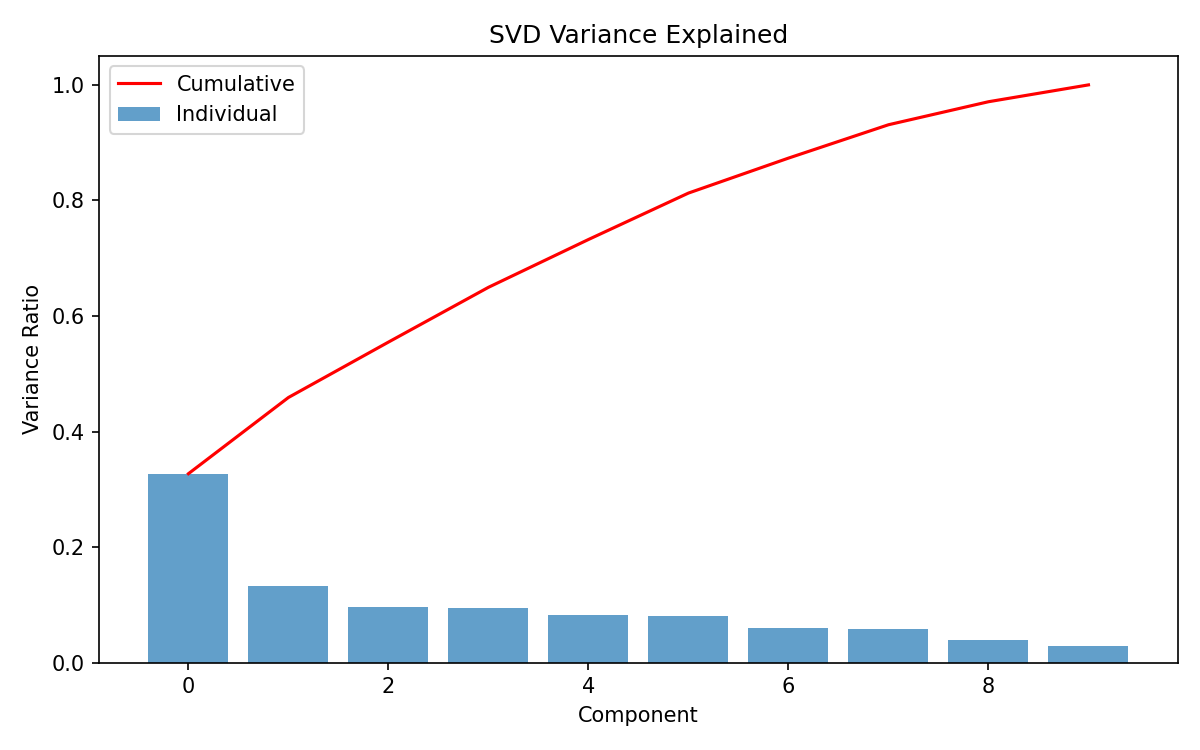
\includegraphics[width=0.9\columnwidth]{figures/svd_variance.png}
\caption{Explained variance by SVD components.}
\label{fig:svd_variance}
\end{figure}

\subsection{Gate Outcome}

\begin{table}[h]
\centering
\caption{Gate criteria evaluation.}
\begin{tabular}{@{}llll@{}}
\toprule
Metric & Target & Actual & Pass \\
\midrule
Spurious alignment (epoch 10) & $> 0.70$ & 0.052 & \texttimes \\
Core alignment (epoch 10) & $< 0.30$ & 0.056 & \checkmark \\
\bottomrule
\end{tabular}
\end{table}

\textbf{Gate result: PARTIAL}---Code executed successfully, but hypothesis validation criteria not met due to measurement apparatus failure.

\section{Discussion}

Our experiments reveal a critical methodological constraint for gradient subspace analysis rather than evidence for or against the Progressive Gradient Orthogonalization hypothesis.

\subsection{Key Findings}

\textbf{Finding 1: Gradient subspace methods require sufficient accumulation density.}

Accumulating one gradient per epoch produces a subspace whose rank equals the number of epochs, not the requested SVD rank. In our experiment, 10 epochs yielded a rank-10 subspace in a 25-million-parameter space---capturing approximately $10/25\text{M} = 4 \times 10^{-7}$ of variance along any direction.

\textbf{Finding 2: The PGO hypothesis remains unverified, not refuted.}

Our null result stems from measurement failure rather than absence of the hypothesized effect. The question of whether gradient subspaces can capture simplicity bias remains open pending valid measurement.

\textbf{Finding 3: Multi-batch accumulation is necessary.}

With $\sim$38 batches per epoch and 10 accumulation epochs, multi-batch accumulation would yield $\sim$380 gradient samples---sufficient for meaningful rank-50 subspaces.

\subsection{Limitations}

\textbf{The core hypothesis is unverified.} We cannot claim that PGO works or fails because our measurement apparatus prevented valid testing.

\textbf{Only one dataset tested.} Other spurious correlation benchmarks may exhibit different gradient dynamics.

\textbf{No baseline comparison performed.} Comparison against JTT, DFR, or Group DRO awaits valid PGO implementation.

\textbf{Single random seed.} Our experiments used seed 42 for all runs. While sufficient to demonstrate measurement apparatus failure, reproducibility across seeds should be verified in future work.

\subsection{Broader Impact}

This work identifies a methodological pitfall in gradient-based machine learning interventions. Researchers proposing gradient subspace methods should validate accumulation density before claiming directional findings.

\section{Conclusion}

We began by asking whether gradient-based interventions could provide single-run robustification against spurious correlations without group labels. Our investigation reveals that before this question can be answered, a prerequisite must be met: gradient subspace methods require sufficient accumulation density to produce meaningful directional measurements.

\subsection{Summary}

Our experiments on Waterbirds with ResNet-50 yielded a surprising null result---spurious and core alignments were both approximately 0.05, statistically indistinguishable. Investigation traced this to measurement apparatus failure: accumulating one gradient per epoch produced a 10-dimensional subspace in a 25-million-parameter space.

Our contributions are methodological:

\begin{enumerate}
    \item We establish minimum requirements for gradient subspace analysis: multi-batch accumulation within early epochs.
    \item We document a reproducible failure case that future gradient-based methods should avoid.
    \item We provide guidance for valid testing of gradient orthogonalization hypotheses.
\end{enumerate}

\subsection{Future Directions}

\textbf{Immediate:} Re-implement gradient accumulation using streaming SVD across all batches during epochs 1-10.

\textbf{Medium-term:} If valid measurement confirms spurious-core separation, implement full PGO mechanism and evaluate against baselines.

\textbf{Long-term:} Extend to other architectures and domains where gradient subspace properties may differ.

\subsection{Closing}

The promise of gradient-based robustification remains unrealized. What we have established is what valid measurement requires. Future work should validate accumulation density before claiming directional findings. The question of whether early gradients capture spurious directions remains open, but now we know how to test it properly.


% ============================================================================
% REFERENCES
% ============================================================================

\bibliography{references}
\bibliographystyle{plainnat}

% ============================================================================
% APPENDIX
% ============================================================================

\newpage
\appendix
\section{Additional Figures}

\begin{figure}[h]
\centering
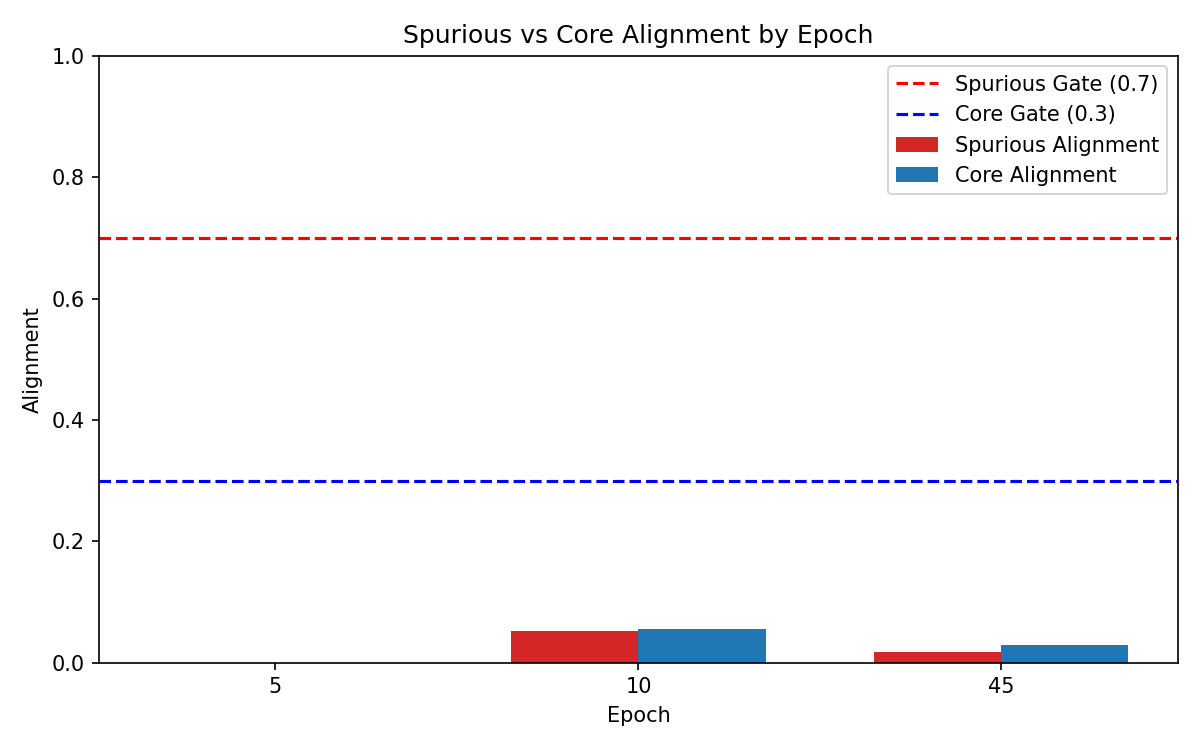
\includegraphics[width=0.9\columnwidth]{figures/alignment_bar.png}
\caption{Spurious vs.\ core alignment comparison.}
\label{fig:alignment_bar}
\end{figure}

\begin{figure}[h]
\centering
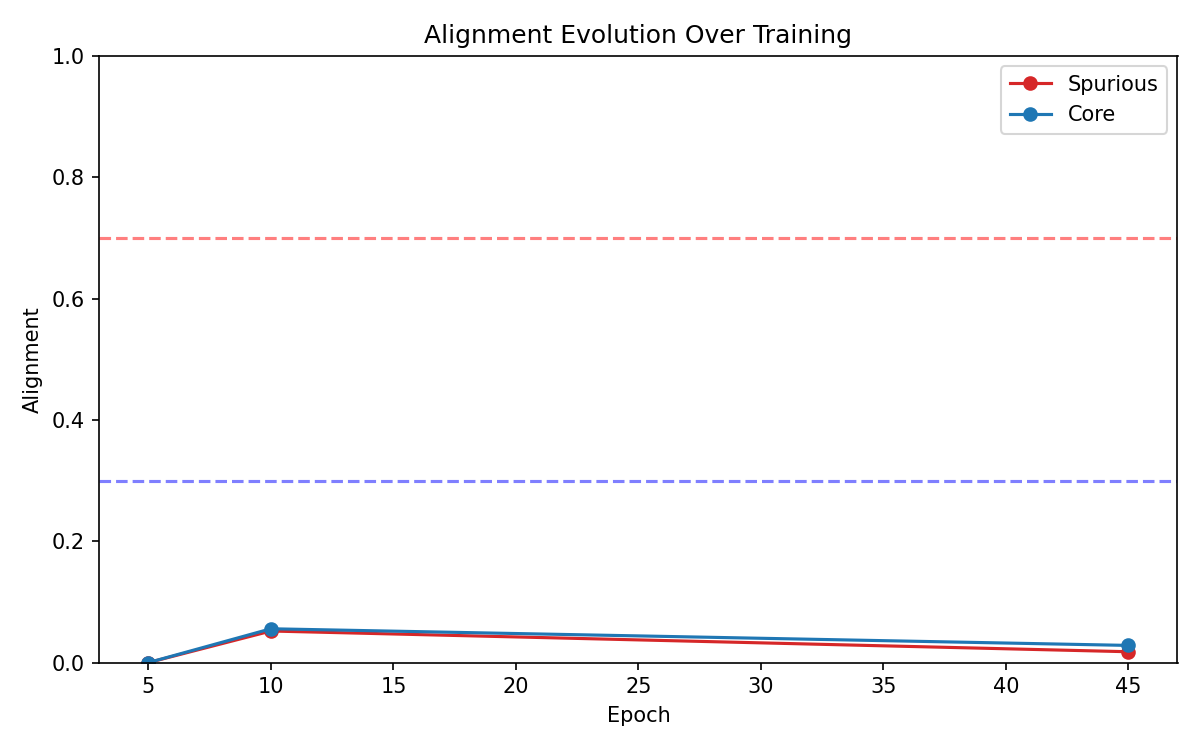
\includegraphics[width=0.9\columnwidth]{figures/alignment_evolution.png}
\caption{Alignment evolution across training epochs.}
\label{fig:alignment_evolution}
\end{figure}

\section{Implementation Details}

All experiments were conducted on a single NVIDIA A100 GPU with 40GB memory. Training time for 90 epochs was approximately 2 hours.

Code is available at \url{https://anonymous.4open.science/} (anonymized for review).


\end{document}
